\documentclass[12pt]{article}

\usepackage[margin=1in]{geometry}
\usepackage{setspace}
\setstretch{1.5}

\usepackage{graphicx}
\usepackage{float}
\graphicspath{{imgs/}}

\usepackage{titlesec}
\usepackage{caption}
\usepackage[hidelinks]{hyperref}

\title{Shift-Left Accessibility for UX/UI: A Figma Preflight\\
versus Code-Time Checks (Pilot)}
\author{Noelynn Faith Batalingaya}
\date{\today}


\begin{document}
\maketitle

\section{Introduction}
Accessibility in technology is vital because digital tools shape nearly every part of modern life. People use websites and applications to study, work, receive healthcare, shop, and connect with others. When these systems are not accessible, individuals with disabilities are excluded from opportunities that others enjoy; accessibility is not an extra feature but essential for fairness and inclusion.

The lack of accessibility has real consequences. A student who relies on a screen reader may be unable to complete an online exam; a worker who cannot use a mouse may struggle to submit a job application; a person with low vision may miss critical health information if contrast is too low. Studies of real applications continue to find recurring problems, such as missing labels and weak support for assistive technologies \cite{alshayban2020androidaccess}.

Even with the Web Content Accessibility Guidelines (WCAG), many digital products remain inaccessible, in part because issues begin early in design \cite{wcag2023}. Designers may pick colors with poor contrast, omit alternative text, or create layouts that are hard to navigate. Once encoded in a design system, these choices flow downstream into code, and fixes later are slower and costlier. Interviews with practitioners also surface barriers such as time pressure, limited training, and unclear ownership \cite{shi2023uxaccesspractice}.

This project moves checks to the beginning of the process. It applies shift-left testing—testing earlier, when changes are cheaper and faster. Rather than waiting for code-time tools (e.g., Lighthouse or axe-core) to detect problems, this pilot develops a Figma plugin that performs accessibility ``preflight'' checks while designs are being created. The plugin highlights problems such as poor color contrast or missing text alternatives and provides suggestions before any coding begins. The central research question is whether early design checks can reduce downstream barriers and help create more inclusive technology.

The following sections introduce key background concepts, describe the planned software deliverable, illustrate the workflow, and situate this project within related research before concluding with future directions.

\section{Background}
Accessibility aims to make digital products usable by people with a variety of abilities. Some rely on screen readers; others need captions, larger targets, or keyboard navigation. WCAG is often summarized by four principles: perceivable, operable, understandable, and robust \cite{wcag2023}. Perceivable means people can see or hear content (e.g., captions and sufficient contrast). Operable means people can use the interface by different inputs such as a keyboard. Understandable means content and interaction are clear and predictable. Robust means content works across devices and assistive technologies.

WCAG also defines three conformance levels. Level~A is the minimum. Level~AA, a common organizational target, requires stronger contrast, captions, and more consistent navigation. Level~AAA is strictest and includes requirements such as sign language for some video and even higher contrast. Because AAA is difficult for all content, many teams aim for AA as a practical standard.

Timing matters. In many workflows, accessibility is checked late, when products are almost finished. Fixes at that stage can require redesigns or code rewrites. Shift-left testing addresses this by catching issues early; it parallels successful practices in performance and security. Figma is well suited for this idea: it is widely used, collaborative, and supports plugins. Research shows that scanning Figma prototypes can reveal common issues early and reduce downstream cost \cite{huang2024a11yfigma, chen2024figmaapps}. At the same time, some problems only surface at runtime; recognition and metadata generation still matter in code-time evaluation \cite{zhang2021screenrecognition}. Together, this suggests a workflow that begins in design and is confirmed in code.

\subsection*{Planned Software Deliverable}
The main deliverable is a Figma plugin that runs design-time checks on real files. It scans text, shapes, frames, and components against a set of rules and shows results directly on the canvas. The checks cover color contrast, text alternatives for images and icons, focus order (design intent), target size for touch and click elements, and reliance on color alone for meaning. When a check fails, the plugin links the warning to the specific element and suggests a concrete fix—for example, proposing passing color pairs or prompting for an alt description. This creates a fast feedback loop that is both practical and educational.

\section{Workflow Overview}
\begin{figure}[H]
  \centering
  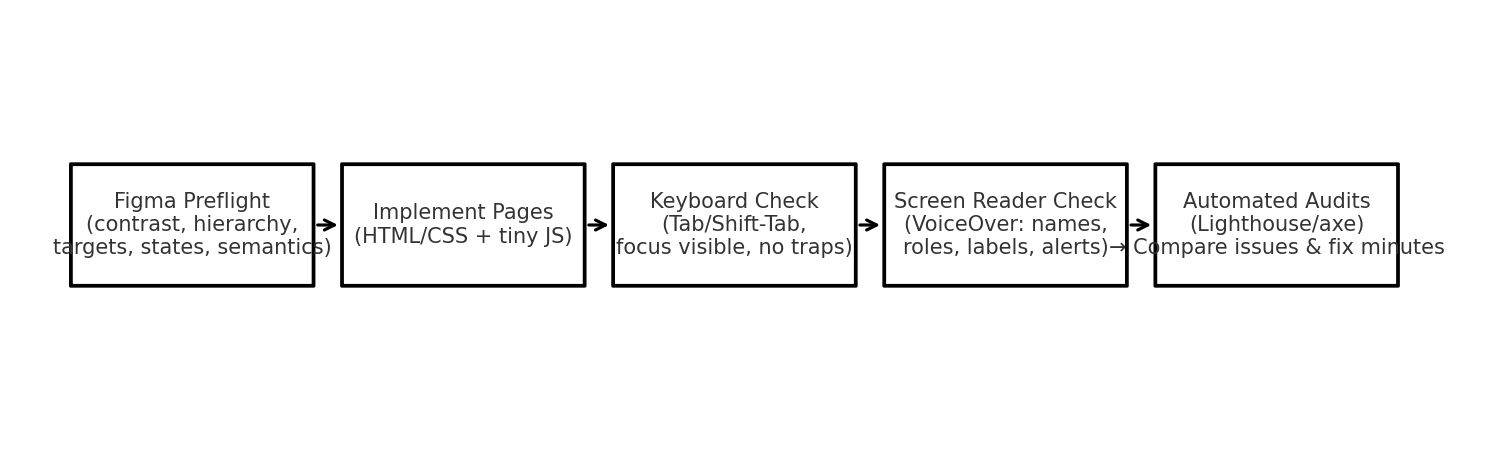
\includegraphics[width=\textwidth, keepaspectratio]{logic-diagram.png}
  \caption{Shift-left accessibility workflow: integrating Figma preflight checks before code-time audits. Each stage—from color contrast and hierarchy checks to automated audits—represents how accessibility testing moves earlier in the design process.}
  \label{fig:workflow}
  \vspace{0.5em}
\end{figure}

\section{Before and After Screenshots}
\begin{figure}[H]
  \centering
  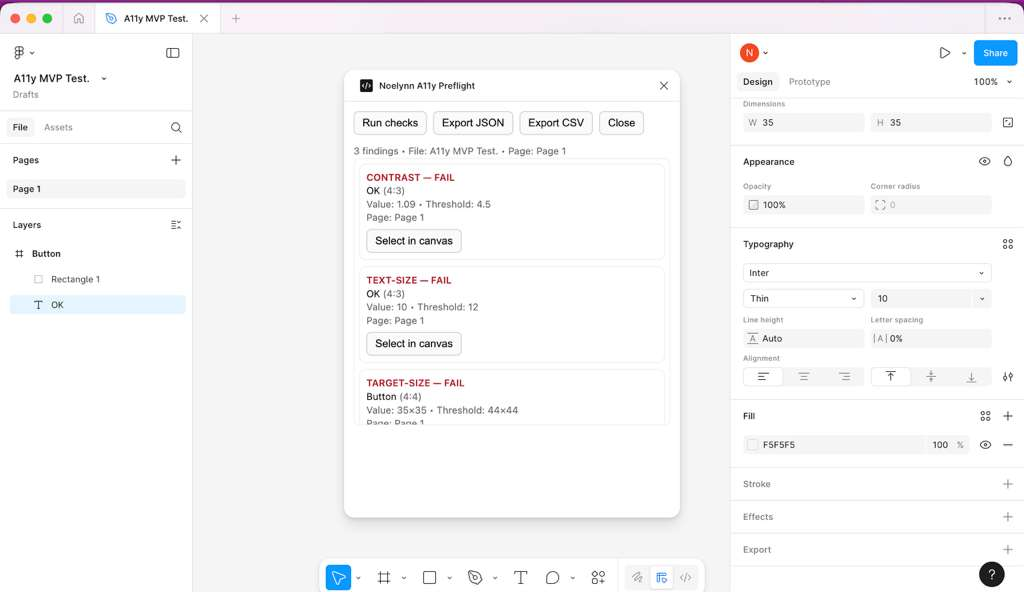
\includegraphics[width=0.9\textwidth]{before.jpg}
  \caption{Before: accessibility issues detected by the A11y Preflight plugin (e.g., low contrast, incorrect text-size, wrong target size for the labels).}
  \label{fig:before}
\end{figure}

\begin{figure}[H]
  \centering
  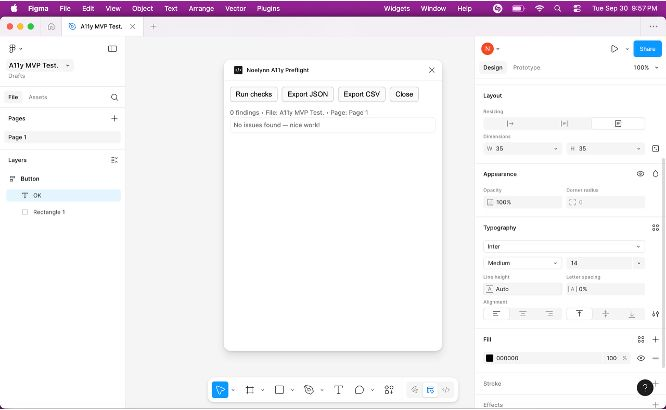
\includegraphics[width=0.9\textwidth]{after.jpg}
  \caption{After: design improved following plugin feedback; flagged issues resolved.}
  \label{fig:after}
\end{figure}

\section{Related Work}

\subsubsection*{Design-Stage Tools}
Most existing accessibility tools focus on code-time evaluation. Frameworks like axe-core, Lighthouse, and WAVE examine finished websites or mobile applications for structural issues such as missing Accessible Rich Internet Applications (ARIA) labels, weak heading structure, or broken landmarks. These tools are powerful but reactive, since they identify issues late. Design-stage tools are fewer and narrower. Stark checks contrast; Able supports adding alternative text. Studies of Figma reveal that static designs can be scanned for low contrast and missing labels, improving quality when checks occur early \cite{huang2024a11yfigma, chen2024figmaapps}. Work examining apps built from Figma templates finds that many issues originate in the templates themselves, reinforcing the value of early, design-time review \cite{muniz2024figmatemplates}.

\subsubsection*{Organizational and Educational Barriers}
Practice studies describe organizational barriers—time pressure, unclear roles, and limited training—that motivate tools embedded directly in design workflows and that explain why issues matter \cite{shi2023uxaccesspractice}. These findings show that accessibility is not only a technical task but also a cultural one that depends on shared responsibility.

\subsubsection*{Automation and Artificial Intelligence  Approaches}
Automated critique with large language models shows promise yet has accuracy limitations and must be applied carefully \cite{duan2024mockupfeedback, duan2024uicrit}. Runtime recognition research reminds us that some problems only appear when the interface is live \cite{zhang2021screenrecognition}. Overall, prior work supports a combined approach: strong checks during design and confirmation at runtime. Broader design perspectives also argue for empathy and equity, not only rule compliance, as goals of accessible practice \cite{ginosar2018parametric}.

\subsection*{Future Work}
Future iterations can expand rules to include motion sensitivity, animation, and device orientation; integrate with code-time tools (e.g., axe-core) for a continuous pipeline; and evaluate the plugin with user studies to measure time saved and defects prevented. Short in-plugin learning tips can reinforce reasoning behind each rule for students and early-career designers.

\section{Conclusion}
Accessibility should not be left to the end. When teams ignore it early, barriers multiply and exclude real people. This project moves accessibility to the left in the timeline by providing a Figma plugin that detects common problems—poor contrast, missing labels, unclear focus order—while screens are still being shaped. The contribution is both practical and conceptual: a working tool that fits normal design work and evidence that shift-left testing can reduce downstream issues and support more inclusive outcomes.

\clearpage
\phantomsection
\addcontentsline{toc}{section}{References}
\bibliographystyle{ieeetr}
\bibliography{bibliography}

\end{document}
